\documentclass[journal,12pt,onecolumn]{IEEEtran}

\usepackage{amsmath,amssymb,amsfonts,amsthm}
\usepackage{graphicx}
\usepackage{enumitem}
\usepackage[breaklinks=true]{hyperref}
\usepackage{caption}
\usepackage{array}
\newtheorem{problem}{Problem}
\renewcommand{\thefigure}{\theenumi}
\renewcommand{\thetable}{\theenumi}
\usepackage{multicol}
\usepackage{amsmath}
\usepackage{gvv}

\begin{document}

\title{GATE EC 2010 - Selected Questions}
\author{AI25BTECH11003 - Bhavesh Gaikwad}
\maketitle

\section*{Electronics and Communication Engineering}

\begin{enumerate}

\item The eigenvalues of a skew-symmetric matrix are
\begin{multicols}{2}
\begin{enumerate}
\item always zero
\item always pure imaginary
\item either zero or pure imaginary
\item always real
\end{enumerate}
\end{multicols}

\item The trigonometric Fourier series for the waveform $f(t)$ shown below contains
\begin{figure}[htbp]
    \centering
    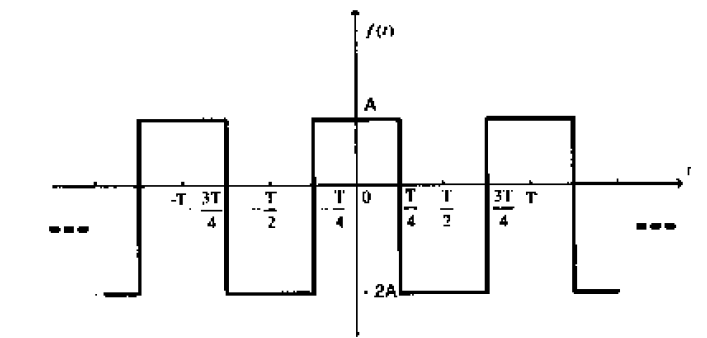
\includegraphics[width=0.3\columnwidth]{figs/fig1.png}
    \caption{Waveform}
    \label{fig:figs/fig1.png}
\end{figure}
\begin{multicols}{2}
\begin{enumerate}
\item only cosine terms and zero value for the dc component
\item only cosine terms and a positive value for the dc component
\item only cosine terms and a negative value for the dc component
\item only sine terms and a negative value for the dc component
\end{enumerate}
\end{multicols}

\item A function $n(x)$ satisfies the differential equation $\frac{d^2 n(x)}{dx^2} = \frac{n(x)}{L^2}$ where $L$ is a constant. The boundary conditions are: $n(0) = K$ and $n(\infty) = 0$. The solution to this equation is
\begin{multicols}{2}
\begin{enumerate}
\item $n(x) = K \exp(x/L)$
\item $n(x) = K \exp(-x/L)$
\item $n(x) = K \exp(-x/L)$
\item $n(x) = K \exp(-x/L)$
\end{enumerate}
\end{multicols}

\item For the two-port network shown below, the short-circuit admittance parameter matrix is
\begin{multicols}{2}
\begin{enumerate}
\item $S=\myvec{4 & -2\\ -2 & 4}$
\item $S= \myvec{1 & 0.5\\ 0.5 & 1}$
\item $S=\myvec{0.5 & 0.5\\ 0.5 & 0.5}$
\item $S=\myvec{2 & -0.5\\ -0.5 & 2}$
\end{enumerate}
\end{multicols}

\item For a parallel RLC circuit, which one of the following statements is NOT correct?
\begin{multicols}{2}
\begin{enumerate}
\item The bandwidth of the circuit decreases if $R$ is increased
\item The bandwidth of the circuit remains same if $L$ is increased
\item At resonance, input impedance is a real quantity
\item At resonance, the magnitude of input impedance attains its minimum value
\end{enumerate}
\end{multicols}

\item At room temperature, a possible value for the mobility of electrons in the inversion layer of a silicon n-channel MOSFET is
\begin{multicols}{2}
\begin{enumerate}
\item 450 cm$^2$/V-s
\item 1350 cm$^2$/V-s
\item 1800 cm$^2$/V-s
\item 3600 cm$^2$/V-s
\end{enumerate}
\end{multicols}

\item Thin gate oxide in a CMOS process is preferably grown using
\begin{multicols}{2}
\begin{enumerate}
\item wet oxidation
\item dry oxidation
\item epitaxial deposition
\item ion implantation
\end{enumerate}
\end{multicols}

\item In the silicon BJT circuit shown below, assume that the emitter area of transistor $Q_1$ is half that of transistor $Q_2$. The value of current $I_0$ is approximately
\begin{multicols}{2}
\begin{enumerate}
\item 0.5 mA
\item 2 $\mu$A
\item 9.3 mA
\item 15 mA
\end{enumerate}
\end{multicols}

\item The amplifier circuit shown below uses a silicon transistor. The capacitors $C_E$ and $C_C$ can be assumed to be short at signal frequency and the effect of output resistance $r_o$ can be ignored. If $C_B$ is disconnected from the circuit, which one of the following statements is TRUE?
\begin{multicols}{2}
\begin{enumerate}
\item The input resistance $R_i$ increases and the magnitude of voltage gain $A_v$ decreases
\item The input resistance $R_i$ decreases and the magnitude of voltage gain $A_v$ increases
\item Both input resistance $R_i$ and the magnitude of voltage gain $A_v$ decrease
\item Both input resistance $R_i$ and the magnitude of voltage gain $A_v$ increase
\end{enumerate}
\end{multicols}

\item Assuming the OP-AMP to be ideal, the voltage gain of the amplifier shown below is
\begin{multicols}{2}
\begin{enumerate}
\item $-\dfrac{R_2}{R_1}$
\item $-\dfrac{R_2}{R_3}$
\item $\left(\dfrac{R_2}{R_1}\right)\left(\dfrac{R_3}{R}\right)$
\item $\left(\dfrac{R}{R_1}\right)\left(\dfrac{R_3}{R_2}\right)$
\end{enumerate}
\end{multicols}

\item Match the logic gates in Column A with their equivalents in Column B.\\


\begin{multicols}{2}
\begin{enumerate}
\item P-2, Q-4, R-1, S-3
\item P-4, Q-2, R-1, S-3
\item P-2, Q-4, R-3, S-1
\item P-4, Q-2, R-3, S-1
\end{enumerate}
\end{multicols}

\item For the output F to be 1 in the logic circuit shown, the input combination should be
\begin{multicols}{2}
\begin{enumerate}
\item $A=1, B=1, C=0$
\item $A=1, B=0, C=0$
\item $A=0, B=1, C=0$
\item $A=0, B=0, C=1$
\end{enumerate}
\end{multicols}

\item In the circuit shown, the device connected to $Y_5$ can have address in the range
\begin{multicols}{2}
\begin{enumerate}
\item 2000-20FF
\item 2000-2DFF
\item 2000-2EFF
\item FD00-FDFF
\end{enumerate}
\end{multicols}

\item Consider the transform $X(z)=5z^2+4z^{-1}+3; 0<|z|<\infty$. The inverse z-transform $x[n]$ is
\begin{multicols}{2}
\begin{enumerate}
\item $5\delta[n+2]+3\delta[n]+4\delta[n-1]$
\item $5\delta[n-2]+3\delta[n]+4\delta[n+1]$
\item $5u[n+2]+3u[n]+4u[n-1]$
\item $5u[n-2]+3u[n]+4u[n+1]$
\end{enumerate}
\end{multicols}

\item Two discrete time systems with impulse responses $h_1[n]=\delta[n-1]$ and $h_2[n]=\delta[n-2]$ are connected in cascade. The overall impulse response of the cascaded system is
\begin{multicols}{2}
\begin{enumerate}
\item $\delta[n-1]+\delta[n-2]$
\item $\delta[n-4]$
\item $\delta[n-3]$
\item $\delta[n-1]\delta[n-2]$
\end{enumerate}
\end{multicols}

\item For an $N$-point FFT algorithm with $N=2^m$, which one of the following statements is TRUE?
\begin{multicols}{2}
\begin{enumerate}
\item It is not possible to construct a signal flow graph with both input and output in normal order
\item The number of butterflies in the $m^{th}$ stage is $N/m$
\item In-place computation requires storage of only $2N$ node data
\item Computation of a butterfly requires only one complex multiplication
\end{enumerate}
\end{multicols}

\item The transfer function $Y(s)/R(s)$ of the system shown is
\begin{multicols}{2}
\begin{enumerate}
\item $\dfrac{1}{s+1}$
\item $\dfrac{1}{s+1}\cdot\dfrac{1}{s+3}$
\item $\dfrac{2}{s+1}$
\item $\dfrac{2}{s+1}\cdot\dfrac{1}{s+3}$
\end{enumerate}
\end{multicols}

\item A system with the transfer function $Y(s)/X(s)=\dfrac{s}{s+p}$ has an output $y(t)=\cos(2t-\pi/3)$ for the input signal $x(t)=p\cos 2t$. Then, the system parameter $p$ is
\begin{multicols}{2}
\begin{enumerate}
\item $\sqrt{3}/2$
\item $\sqrt{3}$
\item 1
\item $2/\sqrt{3}$
\end{enumerate}
\end{multicols}

\item For the asymptotic Bode magnitude plot shown below, the system transfer function can be
\begin{multicols}{2}
\begin{enumerate}
\item $\dfrac{10s+1}{0.1s+1}$
\item $\dfrac{100s+1}{0.1s+1}$
\item $\dfrac{100s}{10s+1}$
\item $\dfrac{10s+1}{0.1s+1}$
\end{enumerate}
\end{multicols}

\item Suppose that the modulating signal is $m(t)=2\cos(2\pi t)$ and the carrier signal $c(t)=A\cos(2\pi f_ct)$. Which one of the following is a conventional AM signal without over-modulation?
\begin{multicols}{2}
\begin{enumerate}
\item $x(t)=A m(t)\cos(2\pi f_c t)$
\item $x(t)=A[1+m(t)]\cos(2\pi f_c t)$
\item $x(t)=A\cos(2\pi f_ct)+m(t)\cos(2\pi f_ct)$
\item $x(t)=A\cos(2\pi f_ct)\cos(2\pi f_ct)+A\sin(2\pi f_ct)\sin(2\pi f_ct)$
\end{enumerate}
\end{multicols}

\item Consider an angle modulated signal $x(t)=6\cos[2\times 10^6\pi t+2\sin(8000\pi t)+4\cos(8000\pi t)]$ V. The average power of $x(t)$ is
\begin{multicols}{2}
\begin{enumerate}
\item 10 W
\item 18 W
\item 20 W
\item 28 W
\end{enumerate}
\end{multicols}

\item If the scattering matrix [S] of a two port network is
$$
[S]=\myvec{0.2\angle 0^\circ & 0.9\angle 90^\circ\\ 0.9\angle 90^\circ & 0.1\angle 90^\circ}
$$
then the network is
\begin{multicols}{2}
\begin{enumerate}
\item lossless and reciprocal
\item lossless but not reciprocal
\item not lossless but reciprocal
\item neither lossless nor reciprocal
\end{enumerate}
\end{multicols}

\item A transmission line has a characteristic impedance of $50\Omega$ and a resistance of $0.1\ \Omega$/m. If the line is distortionless, the attenuation constant (in Np/m) is
\begin{multicols}{2}
\begin{enumerate}
\item 50
\item 5
\item 0.014
\item 0.002
\end{enumerate}
\end{multicols}

\item Consider the pulse shape $s(t)$ as shown. The impulse response $h(t)$ of the filter matched to this pulse is
\begin{multicols}{2}
\begin{enumerate}
\item h(t) diagram A
\item h(t) diagram B
\item h(t) diagram C
\item h(t) diagram D
\end{enumerate}
\end{multicols}

\item The electric field component of a time harmonic plane EM wave traveling in a nonmagnetic lossless dielectric medium has an amplitude of 1 V/m. If the relative permittivity of the medium is 4, the magnitude of the time-average power density vector (in W/m$^2$) is
\begin{multicols}{2}
\begin{enumerate}
\item $\dfrac{1}{30\pi}$
\item $\dfrac{1}{60\pi}$
\item $120\pi$
\item $\dfrac{1}{240\pi}$
\end{enumerate}
\end{multicols}

\item If $y = x^x$, then $y$ has a
\begin{multicols}{2}
\begin{enumerate}
\item maximum at $x=e$
\item minimum at $x=e$
\item maximum at $x=e^{1/e}$
\item minimum at $x=e^{1/e}$
\end{enumerate}
\end{multicols}

\item A fair coin is tossed independently four times. The probability of the event ``the number of times heads show up is more than the number of times tails show up'' is
\begin{multicols}{2}
\begin{enumerate}
\item $1/16$
\item $1/8$
\item $1/4$
\item $5/16$
\end{enumerate}
\end{multicols}

\item If $\vec{A}=xy\ \hat{i}+x\ \hat{j}$, then $\int \vec{A}\cdot d\vec{l}$ over the path shown in the figure is
\begin{multicols}{2}
\begin{enumerate}
\item 0
\item $1/\sqrt{3}$
\item $2/\sqrt{3}$
\item 1
\end{enumerate}
\end{multicols}

\item The residues of a complex function $X(z)=\dfrac{z}{1-z^2}=\dfrac{z}{(z-1)(-z-1)}$ at its poles are
\begin{multicols}{2}
\begin{enumerate}
\item $1/2$ and $1/2$
\item $1/2$ and $-1/2$
\item 1 and $1/2$
\item $5,-1$ and $1/2$
\end{enumerate}
\end{multicols}

\item Consider a differential equation $\dfrac{dy(x)}{dx}-y(x)=x$ with the initial condition $y(0)=0$. Using Euler's first order method with a step size of 0.1, the value of $y(0.3)$ is
\begin{multicols}{2}
\begin{enumerate}
\item 0.01
\item 0.031
\item 0.0631
\item 0.1
\end{enumerate}
\end{multicols}

\item Given $F(s)=\dfrac{3s+1}{s^2+s}$, $f(t)=\mathcal{L}^{-1}\{F(s)\}$ and $F(s)=\dfrac{4}{s^2}+\dfrac{(K-3)}{s}$, $\lim_{t\to\infty} f(t)=1$, then the value of $K$ is
\begin{multicols}{2}
\begin{enumerate}
\item 1
\item 2
\item 3
\item 4
\end{enumerate}
\end{multicols}

\item In the circuit shown, the switch $S$ is open for a long time and is closed at $t=0$. The current $i(t)$ for $t\ge 0$ is
\begin{multicols}{2}
\begin{enumerate}
\item $i(t)=1.5-0.125e^{-1000t}$ A
\item $i(t)=1.5e^{-0.125t-1000t}$ A
\item $i(t)=0.5-0.5e^{-1000t}$ A
\item $i(t)=0.375$ A
\end{enumerate}
\end{multicols}

\item The current $I$ in the circuit shown is
\begin{multicols}{2}
\begin{enumerate}
\item $-j1$ A
\item $j1$ A
\item 0 A
\item 2 A
\end{enumerate}
\end{multicols}

\item In the circuit shown, the power supplied by the voltage source is
\begin{multicols}{2}
\begin{enumerate}
\item 0 W
\item 5 W
\item 10 W
\item 100 W
\end{enumerate}
\end{multicols}

\item In a uniformly doped BJT, assume that $N_e, N_b$ and $N_c$ are the emitter, base and collector dopings in atoms/cm$^3$, respectively. If the emitter injection efficiency of the BJT is close to unity, which one of the following conditions is TRUE?
\begin{multicols}{2}
\begin{enumerate}
\item $N_b N_c$
\item $N_e \gg N_b$ and $N_b > N_c$
\item $N_e N_b$ and $N_b < N_c$
\item $N_e < N_b < N_c$
\end{enumerate}
\end{multicols}

\item Compared to a p-n junction with $N_A=N_D=10^{16}$/cm$^3$, which one of the following statements is TRUE for a p-n junction with $N_A=N_D=10^{20}$/cm$^3$?
\begin{multicols}{2}
\begin{enumerate}
\item Reverse breakdown voltage is lower and depletion capacitance is lower
\item Reverse breakdown voltage is higher and depletion capacitance is lower
\item Reverse breakdown voltage is lower and depletion capacitance is higher
\item Reverse breakdown voltage is higher and depletion capacitance is higher
\end{enumerate}
\end{multicols}

\item Assuming that all flip-flops are in reset condition initially, the count sequence observed at $Q_A$ in the circuit shown is
\begin{multicols}{2}
\begin{enumerate}
\item 0010111...
\item 0001011...
\item 0101011...
\item 0110100...
\end{enumerate}
\end{multicols}

\item The transfer characteristic for the precision rectifier circuit shown below is (assume ideal OP-AMP and practical diodes)
\begin{multicols}{2}
\begin{enumerate}
\item plot A
\item plot B
\item plot C
\item plot D
\end{enumerate}
\end{multicols}

\item The Boolean function realized by the logic circuit shown is
\begin{multicols}{2}
\begin{enumerate}
\item $F=\sum m(0,1,3,5,9,10,14)$
\item $F=\sum m(2,3,5,7,8,12,13)$
\item $F=\sum m(1,2,4,5,11,14,15)$
\item $F=\sum m(2,3,5,7,8,9,12)$
\end{enumerate}
\end{multicols}

\item For the 8085 assembly language program given below, the content of the accumulator after the execution of the program is
\begin{verbatim}
3000 MVI A, 45H
3002 MOV B, A
3003 STC
3004 CMC
3005 RAR
3006 XRA B
\end{verbatim}
\begin{multicols}{2}
\begin{enumerate}
\item 00H
\item 45H
\item 67H
\item E7H
\end{enumerate}
\end{multicols}

\item A continuous time LTI system is described by
$$
\frac{d^2 y(t)}{dt^2}+4\frac{dy(t)}{dt}+3y(t)=2\frac{dx(t)}{dt}+4x(t)
$$
Assuming zero initial conditions, the response $y(t)$ of the above system for the input $x(t)=e^t u(t)$ is given by
\begin{multicols}{2}
\begin{enumerate}
\item $( -e^t) u(t)$
\item $(e^t - e^{-t}) u(t)$
\item $(e^t + e^{-t}) u(t)$
\item $(e^t + e^t) u(t)$
\end{enumerate}
\end{multicols}

\item The transfer function of a discrete time LTI system is given by
$$
H(z)=\frac{1}{(1-\frac{z^{-1}}{2})} - \frac{3}{4}\cdot\frac{1}{(1-\frac{z^{-1}}{2})}
$$
Consider the following statements: S1: The system is stable and causal for ROC: $|z|>2$. S2: The system is stable but not causal for ROC: $|z|<\frac{1}{2}$. S3: The system is neither stable nor causal for ROC: $\frac{1}{2}<|z|<2$. Which one of the following statements is valid?
\begin{multicols}{2}
\begin{enumerate}
\item Both S1 and S2 are true
\item Both S2 and S3 are true
\item Both S1 and S3 are true
\item S1, S2 and S3 are all true
\end{enumerate}
\end{multicols}

\item The Nyquist sampling rate for the signal $s(t)=\dfrac{\sin(500\pi t)}{\pi t}\cdot\dfrac{\sin(700\pi t)}{\pi t}$ is given by
\begin{multicols}{2}
\begin{enumerate}
\item 400 Hz
\item 600 Hz
\item 1200 Hz
\item 1400 Hz
\end{enumerate}
\end{multicols}

\item A unity negative feedback closed loop system has a plant with the transfer function $G(s)=\dfrac{s+2}{s^2+2s} $ and a controller $G_c(s)$ in the feedforward path. For a unit step input, the transfer function of the controller that gives minimum steady state error is
\begin{multicols}{2}
\begin{enumerate}
\item $G_c(s)=\dfrac{s+1}{s+2}$
\item $G_c(s)=\dfrac{s+2}{s+1}$
\item $G_c(s)=\dfrac{(s+1)(s+4)}{(s+2)(s+3)}$
\item $G_c(s)=1+\dfrac{2}{s}+\dfrac{3}{s^2}$
\end{enumerate}
\end{multicols}

\item $X(t)$ is a stationary process with the power spectral density $S_X(f)>0$ for all $f$. The process is passed through a system shown below:
$$
X(t)\ \xrightarrow{\ d/dt\ }\ \text{Delay}=0.5\text{ ms}\ \rightarrow Y(t)
$$
Let $S_Y(f)$ be the power spectral density of $Y(t)$. Which one of the following statements is correct?
\begin{multicols}{2}
\begin{enumerate}
\item $S_Y(f)>0$ for all $f$
\item $S_Y(f)=0$ for $f>1$ kHz
\item $S_Y(f)=0$ for $f=n f_0$, $f_0=2$ kHz, $n$ any integer
\item $S_Y(f)=0$ for $f=(2n+1) f_0$, $f_0=1$ kHz, $n$ any integer
\end{enumerate}
\end{multicols}

\item A plane wave having the electric field component $E=24\cos(3\times 10^8 t - \beta y)\ \hat{a}_x$ V/m and traveling in free space is incident normally on a lossless medium with $\mu_r=4$ and $\epsilon_r=96$ which occupies the region $y\ge 0$. The reflected magnetic field component is given by
\begin{multicols}{2}
\begin{enumerate}
\item $\dfrac{1}{10\pi}\cos(3\times10^8 t + \beta y)\ \hat{a}_z$ A/m
\item $\dfrac{1}{20\pi}\cos(3\times10^8 t + \beta y)\ \hat{a}_z$ A/m
\item $-\dfrac{1}{20\pi}\cos(3\times10^8 t + \beta y)\ \hat{a}_z$ A/m
\item $\dfrac{1}{10\pi}\cos(3\times10^8 t + \beta y)\ \hat{a}_y$ A/m
\end{enumerate}
\end{multicols}

\item In the circuit shown, all the transmission line sections are lossless. The Voltage Standing Wave Ratio (VSWR) on the $60\ \Omega$ line is
\begin{multicols}{2}
\begin{enumerate}
\item 1.00
\item 1.64
\item 2.50
\item 3.00
\end{enumerate}
\end{multicols}

\item Common Data: Consider the common emitter amplifier shown below with the following circuit parameters: $\beta=100$, $g_m=0.3861$ A/V, $r_o=\infty$, $r_\pi=259\ \Omega$, $R_B=1$ k$\Omega$, $R_1=93$ k$\Omega$, $R_E=250\ \Omega$, $R_C=1$ k$\Omega$, $C_1=\infty$ and $C_2=4.7\ \mu$F. The resistance seen by the source $V_s$ is
\begin{multicols}{2}
\begin{enumerate}
\item 258 $\Omega$
\item 1258 $\Omega$
\item 93 k$\Omega$
\item 1 k$\Omega$
\end{enumerate}
\end{multicols}

\item The lower cut-off frequency due to $C_2$ is
\begin{multicols}{2}
\begin{enumerate}
\item 33.9 Hz
\item 27.1 Hz
\item 13.6 Hz
\item 16.9 Hz
\end{enumerate}
\end{multicols}

\item Common Data: The signal flow graph of a system is shown below. The state variable representation of the system can be
\begin{multicols}{2}
\begin{enumerate}
\item $ \dot{x}=\begin{bmatrix}0&1\\ -1&0\end{bmatrix}x+\begin{bmatrix}0\\2\end{bmatrix}u, \ y=[0\ \ 0.5]x $
\item $ \dot{x}=\begin{bmatrix}0&1\\ -1&-1\end{bmatrix}x+\begin{bmatrix}0\\2\end{bmatrix}u, \ y=[0\ \ 0.5]x $
\item $ \dot{x}=\begin{bmatrix}0&1\\ -1&0\end{bmatrix}x+\begin{bmatrix}0\\2\end{bmatrix}u, \ y=[0.5\ \ 0.5]x $
\item $ \dot{x}=\begin{bmatrix}0&1\\ -1&-1\end{bmatrix}x+\begin{bmatrix}0\\2\end{bmatrix}u, \ y=[0.5\ \ 0.5]x $
\end{enumerate}
\end{multicols}

\item The transfer function of the system is
\begin{multicols}{2}
\begin{enumerate}
\item $\dfrac{s+1}{s^2+1}$
\item $\dfrac{s^2+1}{s-1}$
\item $\dfrac{4}{s+1}$
\item $\dfrac{2}{s^2+s+1}$
\end{enumerate}
\end{multicols}

\item Linked Answer: The silicon sample with unit cross-sectional area shown below is in thermal equilibrium. The following information is given: $T=300$ K, electronic charge $=1.6\times 10^{-19}$ C, thermal voltage $=26$ mV and electron mobility $=1350$ cm$^2$/V-s. The magnitude of the electric field at $x=0.5\ \mu$m is
\begin{multicols}{2}
\begin{enumerate}
\item 1 kV/cm
\item 5 kV/cm
\item 10 kV/cm
\item 26 kV/cm
\end{enumerate}
\end{multicols}

\item The magnitude of the electron drift current density at $x=0.5\ \mu$m is
\begin{multicols}{2}
\begin{enumerate}
\item $2.16\times 10^{-1}$ A/cm$^2$
\item $1.08\times 10^{0}$ A/cm$^2$
\item $4.32\times 10^{0}$ A/cm$^2$
\item $6.48\times 10^{2}$ A/cm$^2$
\end{enumerate}
\end{multicols}

\item Consider a baseband binary PAM receiver shown below. The additive channel noise $n(t)$ is white with power spectral density $S_n(f)=N_0/2=10$ W/Hz. The low-pass filter is ideal with unity gain and cutoff frequency 1 MHz. Let $Y$ represent the random variable $y(t)$. $Y=N$ if transmitted bit $b_k=0$, $Y=a+N$ if transmitted bit $b_k=1$ where $N$ represents the noise sample value. The noise sample has a probability density function, $p_N(n)=0.5 a e^{-a|n|}$ (This has mean zero and variance $2/a^2$). Assume transmitted bits to be equiprobable and threshold $z$ is set to $a/2=10$ V. The value of the parameter $a$ (in V$^{-1}$) is
\begin{multicols}{2}
\begin{enumerate}
\item 10
\item $10^2$
\item $1.414\times 10^{-1}$
\item $2\times 10^0$
\end{enumerate}
\end{multicols}

\item The probability of bit error is
\begin{multicols}{2}
\begin{enumerate}
\item $0.5 e^{-1}$
\item $0.5 e^{-2}$
\item $0.5 e^{-7}$
\item $0.5 e^{-10}$
\end{enumerate}
\end{multicols}

\item Which of the following options is the closest in meaning to the word below: Circuitous
\begin{multicols}{2}
\begin{enumerate}
\item cyclic
\item indirect
\item confusing
\item crooked
\end{enumerate}
\end{multicols}

\item The question below consists of a pair of related words followed by four pairs of words. Select the pair that best expresses the relation in the original pair.\\
Unemployed: Worker
\begin{multicols}{2}
\begin{enumerate}
\item fallow: land
\item unaware: sleeper
\item wit: jester
\item renovated: house
\end{enumerate}
\end{multicols}

\item Choose the most appropriate word from the options given below to complete the following sentence: If we manage to \_\_\_\_\_\_ our natural resources, we would leave a better planet for our children.
\begin{multicols}{2}
\begin{enumerate}
\item uphold
\item restrain
\item cherish
\item conserve
\end{enumerate}
\end{multicols}

\item Choose the most appropriate word from the options given below to complete the following sentence: His rather casual remarks on politics \_\_\_\_\_ his lack of seriousness about the subject.
\begin{multicols}{2}
\begin{enumerate}
\item masked
\item belied
\item betrayed
\item suppressed
\end{enumerate}
\end{multicols}

\item 25 persons are in a room. 15 of them play hockey. 17 of them play football and 10 of them play both hockey and football. Then the number of persons playing neither hockey nor football is:
\begin{multicols}{2}
\begin{enumerate}
\item 2
\item 17
\item 13
\item 3
\end{enumerate}
\end{multicols}

\item Modern warfare has changed from large scale clashes of armies to suppression of civilian populations. Chemical agents that do their work silently appear to be suited to such warfare; and regretfully, there exist people in military establishments who think that chemical agents are useful tools for their cause. Which of the following statements best sums up the meaning of the above passage:
\begin{multicols}{2}
\begin{enumerate}
\item Modern warfare has resulted in civil strife.
\item Chemical agents are useful in modern warfare.
\item Use of chemical agents in warfare would be undesirable.
\item People in military establishments like to use chemical agents in war.
\end{enumerate}
\end{multicols}

\item If 137 + 276 = 435 how much is 731 + 672?
\begin{multicols}{2}
\begin{enumerate}
\item 534
\item 1403
\item 1623
\item 1513
\end{enumerate}
\end{multicols}

\item 5 skilled workers can build a wall in 20 days; 8 semi-skilled workers can build a wall in 25 days; 10 unskilled workers can build a wall in 30 days. If a team has 2 skilled, 6 semi-skilled and 5 unskilled workers, how long will it take to build the wall?
\begin{multicols}{2}
\begin{enumerate}
\item 200 days
\item 18 days
\item 16 days
\item 15 days
\end{enumerate}
\end{multicols}

\item Given digits 2, 2, 3, 3, 3, 4, 4, 4, 4 how many distinct 4 digit numbers greater than 3000 can be formed?
\begin{multicols}{2}
\begin{enumerate}
\item 50
\item 51
\item 52
\item 54
\end{enumerate}
\end{multicols}

\item Hari (H), Gita (G), Irfan (I) and Saira (S) are siblings (ie. brothers and sisters). All were born on 1 January. The age difference between any two successive siblings (that is born one after another) is less than 3 years. Given the following facts: (i) Hari's age + Gita's age > Irfan's age + Saira's age. (ii) The age difference between Gita and Saira is 1 year. However, Gita is not the oldest and Saira is not the youngest. (iii) There are no twins. In what order were they born (oldest first)?
\begin{multicols}{2}
\begin{enumerate}
\item HSIG
\item SCHI
\item IGSH
\item IHSG
\end{enumerate}
\end{multicols}

\end{enumerate}

\end{document}
